%% question-4.tex
%%

%% ==============================
\subsection{Diagramme d'objet d'un niveau}
\label{sec:question-4}
%% ==============================

La propriété du jeu qui n'est pas satisfaite par ce niveau est celle de l'accesibilité du coffre par le joueur. En effet dans ce niveau, il n'est pas possible au joueur d'atteindre le coffre.

Le diagramme d'objet suivant décrit le niveau à la figure 3:

\begin{figure}[h!]
	\centering
	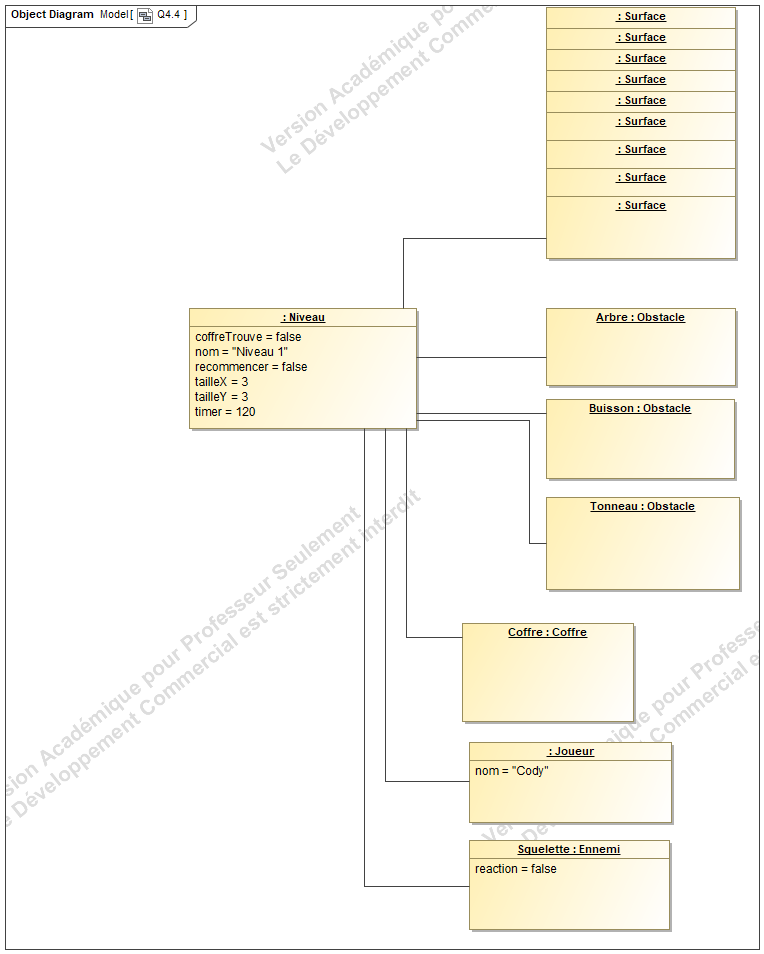
\includegraphics[width=350pt]{assets/Diagramme_objet}
	\caption{Diagramme d'objet de la figure 4.4}
	\label{fig:diagrammeobjet}
\end{figure}

\newpage